\documentclass[11pt,a4paper,ngerman]{article}
\usepackage[bottom=2.5cm,top=2.5cm]{geometry} 
\usepackage{babel}
\usepackage[utf8]{inputenc} 
\usepackage[T1]{fontenc} 
\usepackage{ae} 
\usepackage{amssymb} 
\usepackage{amsmath} 
\usepackage{graphicx}
\usepackage{fancyhdr}
\usepackage{fancyref}
\usepackage{listings}
\usepackage{xcolor}
\usepackage{paralist}
\usepackage{subfigure}

%\usepackage[pdftex, bookmarks=false, pdfstartview={FitH}, linkbordercolor=white]{hyperref}
\usepackage{fancyhdr}
\pagestyle{fancy}
\fancyhead[C]{CoMa II}
\fancyhead[L]{Übung Nr. 9}
\fancyhead[R]{SoSe 2012}
\fancyfoot{}
\fancyfoot[L]{}
\fancyfoot[C]{\thepage / \pageref{LastPage}}
\renewcommand{\footrulewidth}{0.5pt}
\renewcommand{\headrulewidth}{0.5pt}
\setlength{\parindent}{0pt} 
\setlength{\headheight}{0pt}

\author{Tutor: Sebastian Scherer}
\date{}
\title{Max Wisniewski , Alexander Steen}

\begin{document}

\lstset{language=Pascal, basicstyle=\ttfamily\fontsize{10pt}{10pt}\selectfont\upshape, commentstyle=\rmfamily\itshape\small, keywordstyle=\rmfamily\bfseries, breaklines=true, frame=single, xleftmargin=3mm, xrightmargin=3mm, tabsize=2}

\maketitle
\thispagestyle{fancy}


%% ------------------------------------------------------
%%                     AUFGABE 1
%% ------------------------------------------------------

\section*{Aufgabe 1}
%% ------------------------------------------------------
%%                     AUFGABE 2
%% ------------------------------------------------------

\section*{Aufgabe 2}

\begin{lstlisting}[language=matlab, numbers=left]
function [ x, t ] = theta_lin(theta, lambda,f, x0, T, tau )
%theta_lin approximiert das AWP
%AWP x' = lambda*x+f, x(0) = x0 mit einem
%aequidistanten Gitter 0 = t0 < t1 < ... < tn = T
%mit Hilfe des Theta-Verfahrens für Eingabe theta.

x(1) = x0;
t = 0:tau:T; %% Gitter mit Abstand tau

for k = 1:size(t,2)-1,
    x(k+1) = ((x(k)*lambda*tau)*(1 - theta) + x(k) + (f((k-1)*tau)*tau)*(1+theta)+ theta*tau*f(k*tau))/(1-tau*lambda*theta);
% f(k*tau) ist f(t_k+1)...
end
end
\end{lstlisting}

Funzt gut! :D

%\begin{figure}[ht!]
%\center
%\subfigure[Plot des expliziten Euler-Verfahrens mit $\tau = 0.1$]{
%	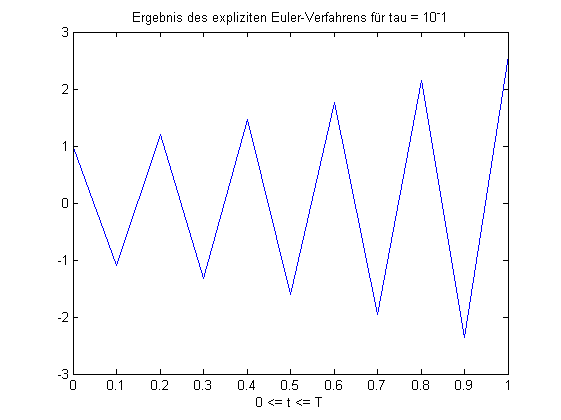
\includegraphics[scale=0.44]{exeuler1.png}
%}
%\subfigure[Plot des expliziten Euler-Verfahrens mit $\tau = 0.01$]{
%	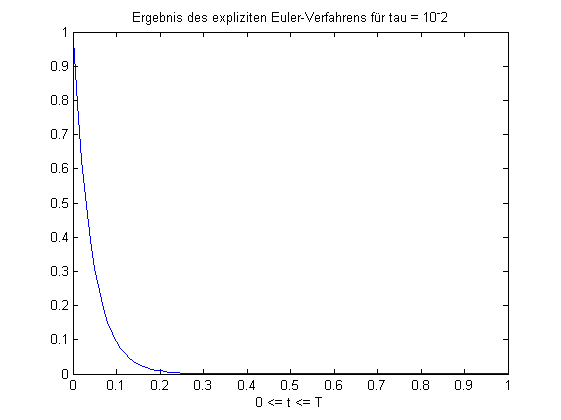
\includegraphics[scale=0.44]{exeuler2.png}
%}
%\subfigure[Plot des expliziten Euler-Verfahrens mit $\tau = 0.001$]{
%	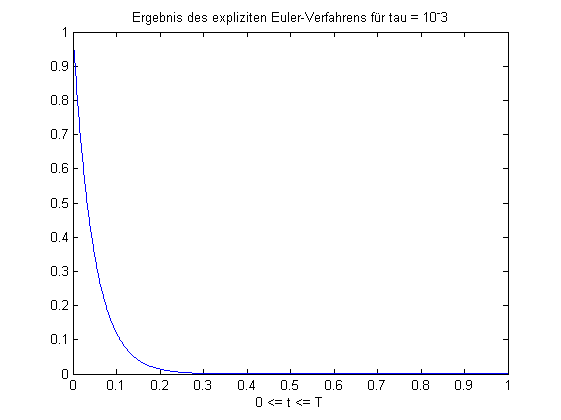
\includegraphics[scale=0.44]{exeuler3.png}
%}
%\end{figure}

%% ------------------------------------------------------
%%                     AUFGABE 3
%% ------------------------------------------------------

%%\section*{Aufgabe 3}


\label{LastPage}

\end{document}
